% =============================================================================
% The CGAL Developers' Manual
% Chapter: Introduction
% -----------------------------------------------------------------------------
% file   : overall_design.tex
% authors: Stefan Schirra <stschirr@mpi-sb.mpg.de>
% -----------------------------------------------------------------------------
% $Id$
% $Date$
% =============================================================================

\section{The overall design\label{sec:overall_design}}
\ccIndexMainItem{design}

The design goals, especially flexibility and efficient robust 
computation, have led us to opt for the generic programming paradigm using 
templates in \CC.\footnote{In appropriate places, however, \cgal\ does 
and should make use of object-oriented solutions and design patterns, as well.}
In the overall design of \cgal\ three major layers can be identified, the
layer of algorithms and data structures, the kernel layer and the
arithmetic and algebra layer.
(Figure~\ref{fig:genericCGAL}).
\ccIndexMainItem{kernel}

\begin{figure}
\begin{ccTexOnly}
\begin{center}
  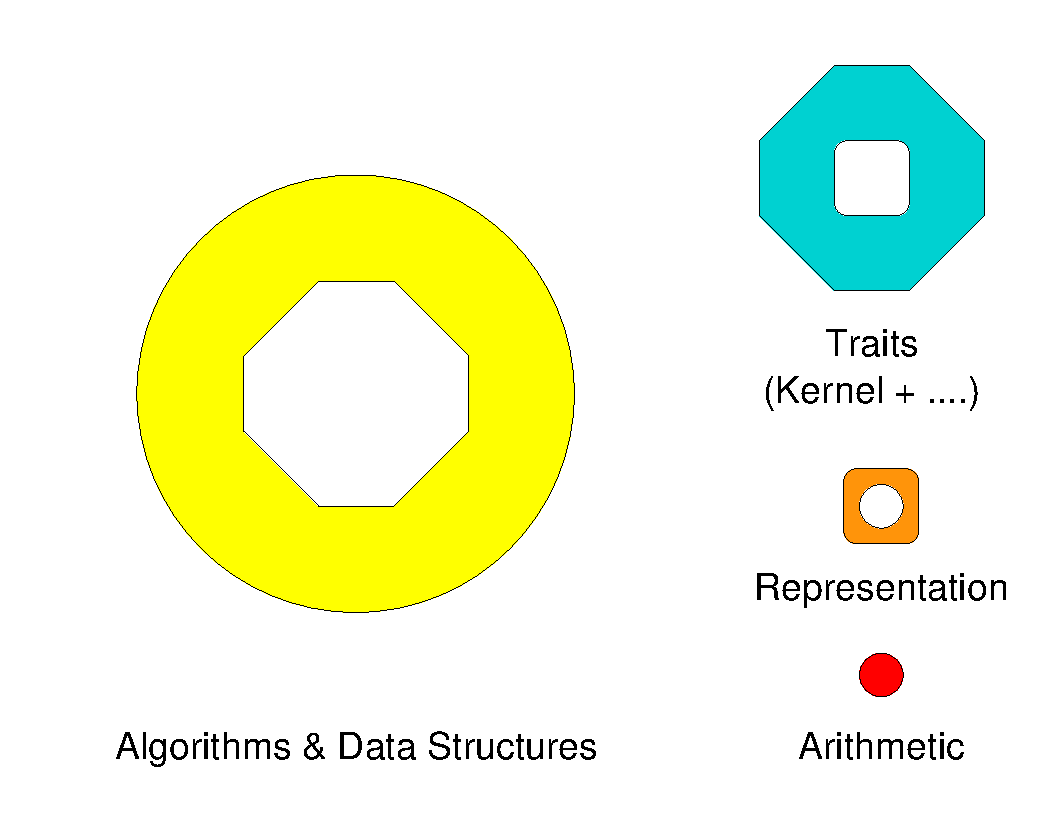
\includegraphics[width=10cm]{Developers_manual/fig/generic_cgal}
\end{center}
\end{ccTexOnly}
\caption{The generic design of \cgal.
\label{fig:genericCGAL}}

\begin{ccHtmlOnly}
<CENTER>
<IMG BORDER=0 SRC="fig/generic_cgal.gif" 
  ALIGN=middle ALT="Generic design of CGAL">
</CENTER>
\end{ccHtmlOnly}
\end{figure}

Algorithms and data structures in \cgal\ are parameterized by the 
types of objects and operations they use. They work with any concrete 
template arguments that fulfill certain syntactical as well as semantic
requirements. In order to avoid long parameter lists,
the parameter types are collected into a single class, called the
traits class in \cgal\ccIndexMainItem{traits class}
(Chapter \ref{chap:traits_classes}.)
A {\em concept}\ccIndexMainItemDef{concepts} is an abstraction of a type 
defined by a set of requirements.
Any concrete type is called a {\em model}\ccIndexMainItemDef{model} for a 
concept if it fulfills
the set of requirements corresponding to the concept. Using this terminology,
we can say a \cgal\ algorithm or data structure comes with a traits 
concept and can be used with any concrete traits model for this concept.
Further contributions to \cgal\ should continue the current high
level of genericity. 

\cgal\ defines the concept of a geometry kernel.%
\ccIndexSubitem{kernel}{concept}
Ideally, any
model for this concept can be used with any \cgal\ algorithm. This holds, 
of course, only if the requirements of an algorithm or data structure on its
traits class are subsumed by the kernel concepts, {\em i.e.}, if an
algorithm or data structure has no special requirements 
not covered in the definition of the kernel concept. Currently, \cgal\
offers a concept for a fundamental geometry kernel, that defines
various geometric objects such as points, line segments, lines,
circles, and operations on them, as well as two additional concepts,
the circular and the spherical kernel. The goal of the last two
kernels is to specify a large set of functionalities on circles and
circular arcs on the plane (circular kernel), and analogous
functionalities for circles, circular arcs living on a 3D sphere
(spherical kernel).

\cgal\ currently provides four models for the \cgal\ 2D and 3D kernel
concept, and one model for the 2D circular and the 3D spherical kernel
concepts.. Those are again parameterized and differ in their 
representation of the geometric objects and the exchangeability of
the types involved. 
In the first four cases the kernels are parameterized by a number type, which
is used to store coordinates and which determines the basic arithmetic
of the kernel primitives.

In the last two cases, the circular and spherical kernel are also
parametrized by Algebraic Kernels, which, along with Algebraic
Foundations, is the third distinct high level of genericity in
\cgal. The algebraic foundations in \cgal\ is a collection of concepts
representing algebraic structures, and are motivated by well-known
counterparts in traditional algebra. The algebraic foundations
determine the operations per algebraic structure, their properties
(e.g., whether they are supposed to be exact or approximate), as well
as interoperability between them.
%
An algebraic kernel is responsible for providing an abstraction
for the algebraic operations required by either geometry kernels or
traits classes used in \cgal\ algorithms. The goal is to be able to
construct, compare and perform operations on real roots of polynomial
equations. There are different concepts depending on the number of
variables of the polynomials used to determine the roots (currently
there are concepts for univariate and bivariate algebraic kernel), as
well as specialized concepts targeted towards specific geometric
higher level layers of the library (such as the circular and spherical
kernels). These concepts are accompanied by at least one model per
concept.

There are further complementary layers in \cgal. The most basic layer is 
the configuration layer.\ccIndexMainItem{configuration layer}
This layer takes care of setting configuration flags according to the outcome
of tests run during installation.  The {\em support library} layer
\ccIndexMainItemDef{support library} is documented in
the \ccAnchor{http://www.cgal.org/Manual/doc_html/frameset/fsSupport.html}{Support Library Reference Manual} and contains packages
that deal with things such as visualization, number types, streams, and
\stl\ extensions in \cgal.

